\begin{savequote}[75mm]
   You know nothing, Jon Snow.
\qauthor{Ygritte, A Song of Ice and Fire by George R. R. Martin}
\end{savequote}

\chapter{Wprowadzenie}
Teoretyczne rozważania dotyczące pochodzenia planet mają długą historię
sięgającą przynajmniej XVIII wieku, kiedy to Immanuel Kant wysunął \dq{}Hipotezę
mgławicową\dq{}. Już wtedy unikalność Układu Słonecznego stanowiła przedmiot
debaty. Dopiero na początku XX wieku pogląd, iż układy planetarne są czymś
powszechnym we Wszechświecie, został zaakceptowany przez środowisko naukowe, a w
roku 1992 została odkryta pierwsza, pozasłoneczna planeta orbitująca pulsar PSR
1257+12 b~\cite{1992Natur.355..145W}.

W połowie XVIII wieku, filozof francuski Immanuel Kant zasugerował, iż rozmyte
o\-biek\-ty obserwowane przez niego przez teleskop mogą być wyspowymi
Wszechświatami takimi jak nasz, bądź obłokami materii w których formują się
gwiazdy i planety~\cite{ImmanuelKant.etal:2008}.

\begin{figure}[!ht]
\centering
%\includegraphics[width=0.8\textwidth]{figures/laplace.png}
\caption{Model mgławicy Laplace'a: (a) rotująca mgławica; (b) kolapsująca
mgławica ulega spłaszczeniu wzdłuż osi rotacji; (c) soczewkowaty kształt
mgławicy; (d) pierścienie materii pozostawione przez zapadający się obiekt
centralny; (e) zagęszczenia na poszczególnych pierścieniach kolapsują tworząc
planety. (Obrazek z pracy Woolfson, 1993)} 
\label{fig:laplace}
\end{figure}

\section{Paradygmat formowania się planet}
Formowanie się planet jest nierozerwalnie związane z narodzinami gwiazd, które
biorą swój początek w gęstych pyłowo--gazowych obłokach materii. Zanurzone w
gorącym ośrodku międzygwiazdowym, początkowo w stanie równowagi termodynamicznej
z otaczającym je gazem, obłoki takie często występują w
ogromnych kompleksach i obserwowane są jako ciemne mgławice molekularne. {\bf
(see Tielens 2005 for a review on a phases of the ISM)} Procesy zachodządze w
samych obłokach, tj. turbulencja, samograwitacja, lub w ośrodku zewnętrznym tj.
wybuchy supernowych mogą powodować wzrost gęstości poszczególnych zagęszczęń w
obłoku. W momencie w którym obszar gęstej materii przekroczy  masę krytyczną,
nazywaną masą Jeansa $M_J$, grawitacja przeważa i chmura zaczyna się zapadać
(rysunek 1a). Masa Jeansa zależy od temperatury kinetycznej ośrodka $T$ oraz
jego gęstości $\rho$ \begin{equation} M_J \sim \left( \frac{k_B T}{G} \right)
^\frac{3}{2} {\rho}^{-\frac{1}{2}}, \end{equation} gdzie $k_B$ jest stałą
Boltzmanna a $G$ jest stałą grawitacji. Dla typowych warunków panujących
wewnątrz obłoków materii międzygwiazdowej, masa Jeansa przyjmuje wartość
\begin{equation}
 M_J \approx 2.9 M_{\odot} \left(\frac{T}{10\K}\right)^{1.5} 
 \left(\frac{n}{10^4\cm^{-3}}\right)^{-0.5},
\end{equation}
gdzie $n = \rho_g / \mu \mH$ jest koncentracją cząstek materii.
Kolaps obłoku następuje w tzw. skali czasowej spadku swobodnego
\begin{equation}
   t_{\textrm{ff}} \sim \frac{1}{\sqrt{G\rho}} \sim 10^5\yr
   \left(\frac{n}{10^4\thinspace \cm^{-3}}\right)^{-0.5},
\end{equation}
co z punktu widzenia całkowitego czasu potrzebnego do uformowania się planet
jest czasem relatywnie krótkim. Podczas kolapsu energia
grawitacyjna zapadającego się obłoku jest przekształcana w energię termiczną.  W
wypadku braku efektywnego mechanizmu chłodzenia się gazu, temperatura wewnątrz
obłoku wzrasta (a wraz z nią masa Jeansa) zatrzymując dalszy kolaps
grawitacyjny. Obserwacyjna klasyfikacja formujacego się układu protoplanetarnego
określa obiekty na tym etapie mianem obiektów \emph{klasy 0}~\cite{andre} (rysunek 1b).
Ich obserwowana temperatura jest stosunkowo niska $(T \lesssim
30\K)$. Obiekty tej klasy charakteryzują się maksimum w
rozkładzie energii promieniowania wypadającym w dalekiej podczerwieni, bez
wykrywalnej nadwyżki w bliskiej podczerwieni.
Kolejnym krokiem ewolucji zapdającego się obłoku jest rozpalenie reakcji
termojądrowych w centrum. Pole promieniowania pochodzące od protogwiazdy
podgrzewa opadająca materię i formujący się dysk do temperatury $T \sim
100\K$ tworząc obiekt \emph{klasy I} (rysunek 1c).  Część
akreująca z dysku materii w pewnym momencie zostaje uniesiona z gwiazdy w
postaci silnego wypływu, który wybija dziurę w otoczce progwiazdowej. Wydarzenie
to może być bardzo gwałtowne i znacznie wpłynąć na tempo akrecji i co za tym
idzie jasność obiektu. Gwałtowny wybuch zwyczajowo nazywa się \emph{rozbłyskiem
FU--Orionis}.
W obiektach \emph{klasy I} maksimum w rozkładzie energii promieniowania przesuwa
się w kierunku bliskiej podczerwieni, praktycznie wypłaszczając widmo.  \par Po
około $10^5$ lat, większość otoczki zostaje odrzucona przez wiatr, a dysk
protogwiazdowy zostaje zredukowany do kilku procent masy gwiazdy macierzystej.
Osiągana jest bardziej stabilna konfiguracja, tzw. faza \emph{T-Tauri} dla
gwiazd o masach mniejszych niż $2\thinspace\Msun$, badź faza \emph{Herbig Ae/Be}
dla gwiazd masywniejszych. Dla obiektów tej klasy (\emph{klasa II} rysunek 1d)
znacznie spada nadwyżka w podczerwieni. Okres ten trwa od $10^5$ do $10^6$ lat.

% Pozniej
%Na tym etapie musi nastąpić formacja planetezymali i gazowych olbrzymów,
%ponieważ po jej zakończeniu dysk protoplanetarny zanika.  Pozostaje gwiazda
%zbliżająca się do ciągu głównego, nie wykazująca już żadnej nadwyżki w
%podczerwieni --- obiekt \emph{klasy III} (rysunek 1e).

\begin{figure}[p]
\centering 
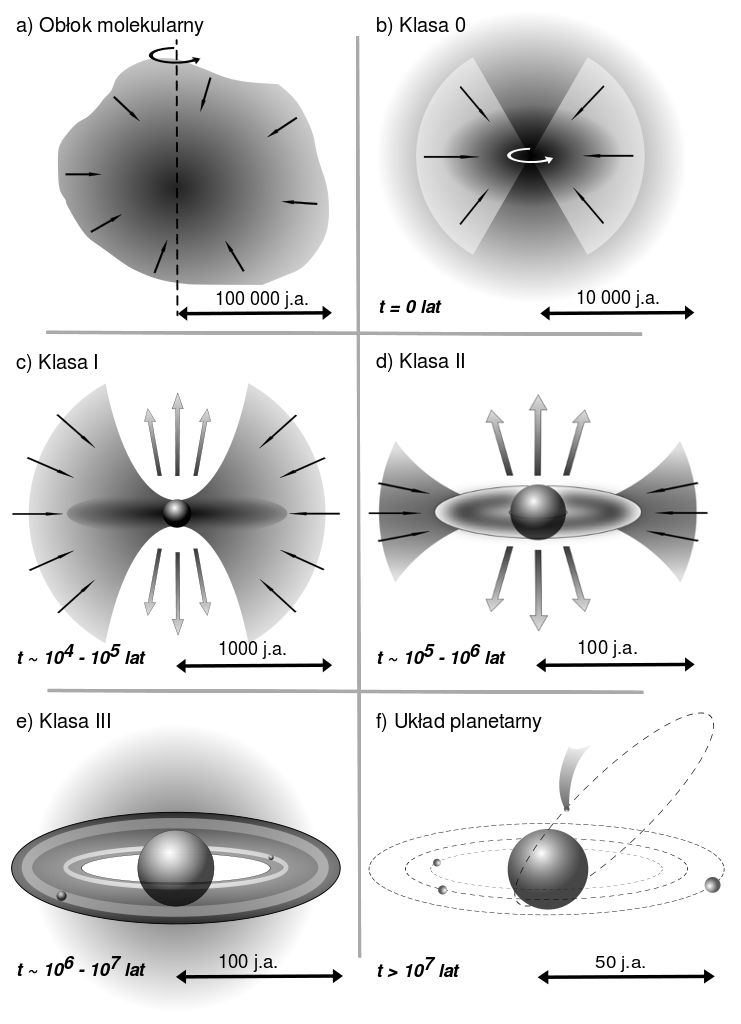
\includegraphics[width=0.9\textwidth]{figures/planetformation.png}
\caption{Ilustracja przedstawia kolejne fazy formowania się małomasywnej gwiazdy
   wraz z systemem planetarnym: a) kolaps grawitacyjny gęstego obłoku; b)
   oddziaływanie centralnego pola grawitacyjnego oraz siły odśrodkowej powoduje
   opadanie materii i formowanie się dysku; c) faza FU Orionis: silna akrecja w
   dysku oraz wypływ materii w okolicach osi obrotu; d) faza T Tauri: zmniejsza
   się tempo akrecji $\sim 10^{-8}\Msun\yt^{-1}$ oraz wypływu materii,
   rozpoczyna się proces formowania planet; e) zanika składowa gazowa, planety
otwierają przerwy w dysku, następuje również ich migracja; f) cały gaz oraz
mniejsze ciała zostają pochłonięte przez planety lub usunięte z dysku, układ
planetarny przyjmuje ostateczny kształt.}

\label{fig:planet}
\end{figure}

%\section{Faza T Tauri}

Podczas tej fazy większość energii wyświecanej przez gwiazdę pochodzi ciągle z
energii grawitacyjnej traconej podczas kontrakcji. Ewolucja zachodzi w tzw.
skali czasowej Kelvina--Helmholtza 

\begin{equation} 
   t_{KH} \sim  \frac{G{M_{\star}}^2}{R_{\star}L_{\star}} = 3\cdot 10^7 \yr
   \left(\frac{M_\star}{M_\odot}\right)^{2}
   \left(\frac{L_\star}{L_\odot}\right)^{-1}
   \left(\frac{R_\star}{R_\odot}\right)^{-1}
\end{equation}

gdzie $M_{\star}$, $R_{\star}$, $L_{\star}$ są odpowiednio masą, promieniem i
dzielnością promieniowania gwiazdy. Formująca się gwiazda powoli przesuwa się na
diagramie Hertzsprunga--Russela w kierunku ciągu głównego wieku
zerowego~\cite{palla}.  Dla gwiazd o masie Słońca ewolucja ta będzie przebiegała
po tzw. ścieżce Hayashiego, na której obiekty pozostają całkowicie konwektywne,
podczas gdy gwiazdy bardziej masywne utworzą promieniste jądra i przesuną się
w stronę wyższych temperatur. W tym czasie otaczający gwiazdę dysk traci
gaz na skutek fotoewaporacji i wiatru gwiazdowego. Zarówno obserwacje gwiazd
T-Tauri jak i rozważania teoretyczne~\cite{alexanderpassuci2013} {\bf and ref
therein} szacują że proces utraty gazu z dysku trwa od jednego do kilku Myr.
Stanowi to niewątpliwie limit na wytworzenie się gazowych olbrzymów, tj. w dysku
protoplanetarnym muszą wcześniej wytworzyć się obiekty zdolne akreaować wodór.

\par Po dyspersji dysku gazowego gwiazda powoli traci również nadwyżkę w
podczerwieni. Sugeruje to fakt, iż skala czasowa koagulacji pyłu w większe
ziarna jest porównywalna z czasem życia frakcji gazowej dysku. Ewolucję pyłu
można podzielić na zgrubsza na 4 etapy:
\begin{description}
   \item[i) koagulacja ziaren pyłu $\left(\mum \rightarrow \km\right):$] 
      Z doświadczeń laboratoryjnych wynika~\cite{me}, że drob\-ne cząsteczki pyłu
      mogą na skutek wzajemnych zderzeń zwiększać swoje rozmiary. ,,Spoiwem'' stają
      się siły van der Waalsa bądź oddziaływanie elektrostatyczne. Opierając się
      na analizie drogi swobodnej jednorodnej frakcji cząstek pyłu o promienu
      $a$, można określić charakterystyczną skalę czasową koagulacji jako 

   \begin{equation}\label{coag} 
      t_{\textrm{coag}} % = \frac{1}{n_d \sigma \Delta v}
      \sim \frac{a}{\Delta v}\frac{\rho_p}{\rho_d} \approx 
      10^{-12} \rho_d^{-1}\yr\thinspace
      \left(\frac{a}{1\mum}\right)
      \left(\frac{\Delta v}{0.1\m\s^{-1}}\right)^{-1}
      \left(\frac{\rho_p}{3\g\cm^{-3}}\right),
   \end{equation}

   gdzie $\Delta v$ jest średnią prędkością względna cząstek, $\rho_p$ jest
   gęstością materiału budującego cząstki natomiast $\rho_d$ jest gęstością
   ośrodka pyłowego w dysku.  Biorąc pod uwagę typowe gęstości pyłu w obłokach
   gwiazdowych $(\rho_d \sim 10^{-20}\g\cm^{-3})$ proces ten
   zachodzi w skali czasowej milionów lat. Jednakże dla dysków protoplanetarnych
   o typowych gęstościach rzędu $10^{-10}\g\cm^{-3}$\footnote{jest to całkowita
   gęstość z uwzględnieniem obu składników: gazu i pyłu. Przyjmuje się że
kanoniczna wartość stosunku gęstości pyłu do gęstości gazu $\epsilon$ wynosi
0.01. Zatem $\rho_d \sim 10^{-12}\g\cm^{-3}$} proces
koagulacji zachodzi w skalach lat czy tez dziesiątek lat i może bardzo szybko
prowadzić do wytworzenia się planetezymali. W rzeczywistości dla ziaren pyłu o
rozmiarach decymetrów czy metrów pojawia się szereg procesów przeciwdziałających
dalszemu wzrostowi, a także ulega zmianie średnia prędkość względna cząstek pyłu
zmieniając prawdopodobnięstwo wyniku kolizji na korzyść fragmentacji raczej niż
koagulacji.  

\item[ii) oligarchiczny wzrost $\left(\km \rightarrow
   10^3\km\right)$:]
   Faza druga formowania się planet rozpoczyna się w momencie w którym przeważa
   wzajemne oddziaływanie grawitacyjne pomiędzy planetezymalami i to grawitacja
   staje się nowym spoiwem łączącym zderzające się obiekty. Tarcie
   aerodynamiczne jest nadal niezaniedbywalne i zapewnia kołowość orbit
   planetezymali, co zwiększa szanse na zderzenia.
\item[iii) akrecja gazu]
   Po osiągnięciu rozmiarów rzędu $10^3\km$ jądra planetarne
   są w stanie wiązać grawitacyjnie gaz na swoich powierzchniach. Globalne
   oddziaływanie dysk $\iff$ planety staje się istotne i może prowadzić z jednej
   strony do migracji planet, a z drugiej strony do otworzenia się przerw w
   dysku.
\item[iv) długoskalowa ewolucja dynamiczna:]
   Faza zdominowana tylko i wyłącznie przez wzajemne oddziaływanie grawitacyjne
   pomiędzy utworzonymi planetami, a także z gwiazdą macierzystą. Układ
   planetarny może na tym etapie utracić znaczną część masy pyłowej, poprzez
   pochłonięcię planety przez gwiazdę, bądź wprowadzenie jej na orbitę
   hiperboliczną.
\end{description}
Powyższy scenariusz formowania się planet nosi nazwę modelu ,,akrecji na
jądra''~\footnote{ang. \emph{core-accretion}}. Alternatywną teorią, szczególnie
wdzięcznie wyjaśniająca powstawanie gazowych olbrzymów w masywnych dyskach
protoplanetarnych, jest model zakładający kolaps i fragmentację grawitacyjną
dysku~\cite{Boss}. Zostanie ona omówiona w dalszej części tego rozdziału.

\section{Ważne pojęcia}
Gazowo--pyłowy dysk, który powstaje podczas kolapsu obłoku protogwiazdowego jest
miejscem w którym powstają planety. Pewne szczególne mechanizmy oraz globalna
dynamika mogą temu procesowi pomagać, bądź mu przeciwdziałać. Poniższe akapity
pokrótce opisują strukturę dysku protoplanetarnego oraz najważniejsze efekty
dynamiczne związane z samym gazem, następnie przechodząc do ich wpływu na
dynamikę i ewolucję pyłu. Pozwoli to wskazać problemy z jakimi boryka się model
,,akrecji na jądra'' i naturalnie przejść do celu tej rozprawy.

\subsection{Struktura dysku protoplanetarnego}
Proces kolapsu grawitacyjnego, sferycznego obłoku materii międzygwiazdowej nie
wpływa na jego całkowity moment pędu. Przy założeniu, że obłok rotuje, nawet
bardzo wolno, to materia nie opada bezpośrednio na obiekt
centralny, lecz formuje dysk w płaszczyźnie prostopadłej do wektora całkowitego
momentu pędu. Aby określić przybliżone warunki fizyczne w formującym się dysku
możemy posłużyć się równaniami hydrodynamiki:

\begin{gather}
   \partial_t \rho_g + \nabla\cdot\left(\rho_g\mathbf{u}\right) = 0,
   \label{eq:hd1}\\
\partial_t \mathbf{u} + \left(\mathbf{u}\cdot\nabla\right)\mathbf{u} = 
-\nabla\Phi + -\frac{1}{\rho_g} \nabla P \label{eq:hd2}
\end{gather}

gdzie $\rho_g$ jest gęstością gazu, $P$ ciśnieniem, 
związanych z tarciem, a $\Phi$ potecjałem grawitacyjnym. Jeżeli ponadto
założymy, że dysk:

\begin{enumerate}
   \item jest izotermiczny to $P = c_s^2 \rho_g \implies -\frac{1}{\rho_g}\nabla
      P = -c_s^2\nabla\ln\rho_g$, gdzie $c_s = \sqrt{\frac{k_{\textrm{B}} T}{\mu
    \mH}}$ jest izotermiczną prędkością dźwięku.
   \item jest stacjonarny i znajduję się w równowadzę hydrostatycznej w kierunku
      $z$ to wertykalne przyspieszenie grawitacyjne $\partial_z \Phi = g_z =
      (GM_\star/r^2) z/r = \Omega^2 z$, gdzie $M_\star$ to masa gwiazdy
      macierzystej, $\Omega$ orbitalna częstość keplerowska, $G$ stała
      grawitacji Newtona, jest równoważone przez siłę wynikająca z gradientu
      ciśnienia gazu $\partial_z P / \rho_g$
\end{enumerate}

Łącząc powyższe założenia otrzymujemy rozkład gęstości gazu

\begin{equation}
   \rho_g(z) = \frac{\Sigma_G}{H\sqrt{2\pi}} \exp \left[
   \frac{1}{2}\left(\frac{z}{H}\right)^2 \right],
\end{equation}

gdzie $\Sigma_g = \int \rho_g(z) dz$ jest gęstością powierzchniową, a
$H=\frac{c_s}{\Omega}$ to charakterystyczna skala grubości dysku.

%\par Zakładając w pierwszym przybliżeniu że dysk jest optycznie gruby, t.j.
%absorbuję całkowicie promieniowanie pochodzące od gwiazdy i następnie reemituje
%je jako ciało doskonale czarne, można pokazać~\cite{armitage07} że $T \propto
%r^{-3/4}$ i co za tym idzie $c_s \propto r^{-3/8}$. Dokładniejsze szacunki,
%które lepiej oddają obserwowane dystrucje spektralne energii, można znaleźć w
%pracach~\cite{KenyonHART87, ChaingGold97} {\bf patrz armitage}.
%{\bf Tu raczej trzeba przedstawić tę wersję z której wynika $T \propto
%r^{-1/2}$}
%
\par W modelu stacjonarnym w kierunku radialnym grawitacja i siła wynikająca z
gradientu ciśnienia jest równoważona poprzez siłę odśrodkową
\begin{equation}\label{eq:radial_balance}
\frac{u_\phi^2}{r} = \frac{GM_\star}{r^2} +
  \frac{1}{\rho_g}\frac{\textrm{d}P}{\textrm{dr}},
\end{equation}
gdzie $u_\phi$ jest prędkością orbitalną gazu. Wpływ gradientu ciśnienia na
globalną dynamikę jest znikomy (rzędu $O(H/r)^2$), dlatego dla cienkich dysków
$(H/r \ll 1)$ z dobrym przybliżeniem można przyjąć, że właściwy moment pędu dla
gazu jest równy momentowi pędu wynikającemu z ruchu keplerowskiego. Z równania
\mref{eq:radial_balance} wynika zatem, że moment pędu jest rosnącą funkcją
promienia:
\begin{equation}\label{eq:angmom}
l = r^2\Omega = \sqrt{GM_\star r}.
\end{equation}
Z równania \mref{eq:angmom} wypływa niezwykle ważny fakt: aby materiał z dysku
mógł być akreaowany przez gwiazdę macierzystą, w układzie musi działać mechanizm
powodujący utratę bądź chociaż redystrybucję momentu pędu.
\subsection{Niestabilność magnetorotacyjna}
Z obserwacji jasno wynika~{\bf cytacja i rysunek 0402599?}, że dyski
protoplanetarne nie są obiektami stacjonarnymi. Co więcej, obiekty klasy I
posiadają wysokie tempa akrecji $\sim 10^{-5}\Msun\yr^{-1}$. Aby zapewnić
radialny przepływ materii w kierunku gwiazdy macierzystej, potrzeba wprowadzić
efektywny mechanizm transportu momentu pędu. W tym celu musimy odejść od
przybliżenia hydrodynamiki dla idealnego gazu i zastować równania
Naviera-Stokesa, które rozszerzają równanie ruchu~\ref{eq:hd2} o tensor naprężeń
płynu

\begin{gather}
   \partial_t \rho_g + \nabla\cdot\left(\rho_g\mathbf{u}\right) = 0,
   \label{eq:ns1}\\
\partial_t \mathbf{u} + \left(\mathbf{u}\cdot\nabla\right)\mathbf{u} = 
-\nabla\Phi -\frac{1}{\rho_g} \nabla P + \frac{1}{\rho_g} \nabla \cdot \Pi.
\label{eq:ns2}
\end{gather}
Jeżeli dodatkowo założymy, że mamy doczynienia z płynem doskonale lepkim, tensor
naprężeń można zredukować do postaci $\Pi = (\rho_g \nu)\nabla\cdot\mathbf{u}$,
gdzie $\nu$ jest lepkością kinematyczną. Całkując układ
równań~\mref{eq:ns1}-\mref{eq:ns2} w kierunku wertykalnym i dokonująć prostych
przekształceń można otrzymać
\begin{equation}\label{eq:sigma}
   \partial_t \Sigma_g =
   \frac{3}{R}\partial_R\left(\frac{1}{R\Omega}\partial_R\left(R^2\Sigma_g \nu
         \Omega\right)\right).
\end{equation}
Rozwiązaniem stacjonarnym równania~\mref{eq:sigma} jest warunek $\Sigma_g\nu =
\textrm{const}$, co przekłada się na tempo akrecji $\dot{M} = 3\pi\Sigma_g\nu$.
Z powyższego warunku wynika, że lepkość jest kluczowym elementem napędzającym
akrecję materii. Problemem pozostaje jakie proces fizyczny jest za nią
odpowiedzialny?
\par Podstawowa lepkość, tj. lepkość molekularna $\nu_{\textrm{m}} \sim c_s
\lambda$, gdzie $\lambda = 1 / n\sigma$ to średnia droga swobodna molekuł gazu,
zaś $n$ to koncetracja molekuł gazu, a $\sigma$ ich przekrój czynny, dla
typowych wartości gęstości i temperatury dysków protoplanetarnych wynosi
$\nu_{\textrm{m}}\sim10^5\cm^2\s^{-1}$~\cite{armitage}. Przekłada się to na
tempo akrecji na poziomie $\dot{M}\sim 10^{-17}\Msun\yr^{-1}$. Co więcej
charakterystyczna skala czasowa takiego procesu $\tau \simeq R^2 /
\nu_{\textrm{m}}$ wynosi $10^{13}\yr$. Z tego względu lepkość molekularną można
całkowicie zaniedbać w dalszych rozważaniach.
\par W słynnej pracy Shakura \& Sunyaev~\citep{SS73} zauważyli, że turbulencja
w dysku może być dobrym źródłem lepkości, znacznie wydajnieszym niż lepkość
molekularna. Dla izotropowej turbulencji, maksymalna skala wirów w dysku jest
proporcjonalna do charakterystycznej skali grubości dysku $H$, zaś maksymalna
prędkość ruchu turbulentnych jest rzędu prędkości dźwięku, ponieważ fale
uderzeniowe bardzo szybko dyssypują energię kinetyczną. Shakura \& Sunyaev
zaproponowali parametryzację lepkości turbulentnej

\begin{equation}\label{eq:alpha}
\nu = \alpha c_s H
\end{equation}

, gdzie $\alpha$ jest bezwymiarowym parametrem określającym wydajność
turbulencji w transporcie momentu pędu. Aby wyjaśnić obserwowane tempo akrecji
dla gwiazd \emph{T Tauri}, parameter $\alpha$ powinnien byc rzędu $10^{-2}$.
Problem dalej pozostaje źródło turbulencji w dysku. Z kryterium
Rayleigha

\begin{equation}
   \frac{\mathrm{d}}{\mathrm{d}r}\left(r^2\Omega\right) > 0,
\end{equation}

wynika że hydrodynamiczny dysk keplerowski jest liniowo stabilny. Sytuacja
diametralnie się zmienia w jeżeli uwzględnimy obecność w układzie dowolnie
słabego pola magnetycznego. Balbus \& Hawley~\citep{BH91} pokazali, że przepływ
magnetohydrodynamiczny jest stabilny liniowo wtedy i tylko wtedy, gdy

\begin{equation}\label{eq:mri}
   \frac{\mathrm{d}}{\mathrm{d}r}\left(\Omega^2\right) > 0.
\end{equation}
Warunek \mref{eq:mri} \emph{nie jest} spełniony dla dysków keplerowskich. W
rezultacie nawet szczątkowe pole magnetyczne, jest w stanie wzmocnić wykładniczo
zaburzenia gęstości w gazie w dynamicznej skali czasowej, powodując silną
turbulencję. Proces ten określany jest mianem niestabilności magnetorotacyjnej
(MRI). Co więcej, zarówno symulacje lokalne~\cite{Davis_Stone_Pessah_2010} jak
i globalne~\cite{Flock} szacują współczynnik $\alpha$ wynikający z turbulencji
wzbudzonej przez MRI na $\alpha\sim 10^{-2}$.

\begin{figure}
   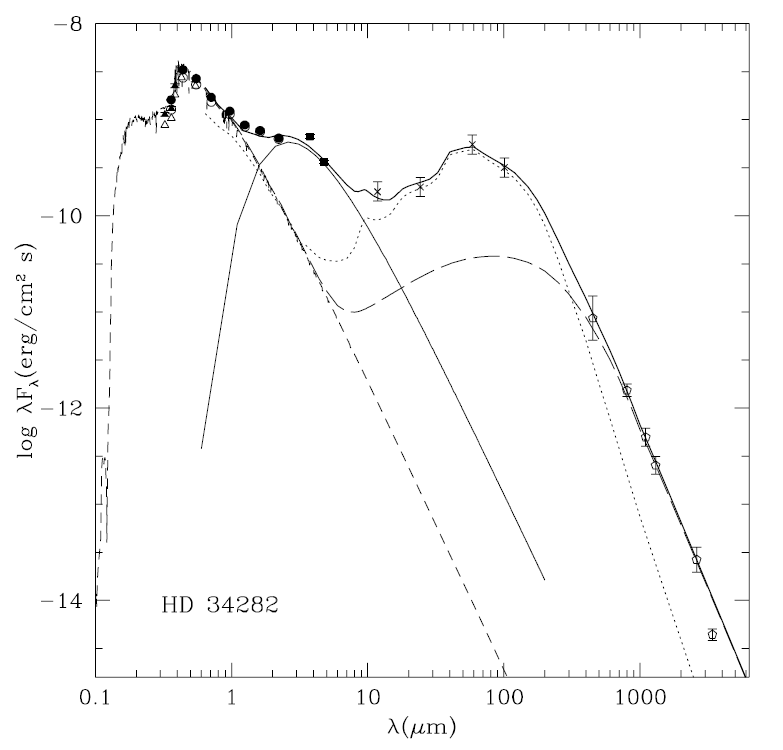
\includegraphics[width=0.9\textwidth]{figures/chap1_sed.png}
   \caption{Rozkład widma energii dla gwiazdy HD 34282. Symbole oznaczają
      obserwacje różnymi metodami dla odpowiednich długości fali. Do obserwacji
      dopasowano następujące modele: linia przerywana model widma gwiazdowego
      dla obiektu typu A3V $(T\sim 8600\K)$, cienka ciągła
      linia model ciała doskonale czarnego dla $T=1400\K$,
      linia kropkowana reprezentuje model dysku o nachyleniu $i=56^o$, tempie
      akrecji $\dot{M} = 8.2\times10^{-9}\thinspace\Msun\yr^{-1}$
      rozciągającym się od $0.31\AU$ do $705\AU$.
   Obrazek pochodzi z pracy~\cite{0402599}}
\end{figure}

\subsection{Niestabilność grawitacyjna}
\subsection{Oddziaływanie pomiędzy gazem, a pyłem}
\subsection{Radialny dryf pyłu}
\subsection{Sedymentacja i pułapkowanie pyłu (KHI)}
\subsection{Koagulacja i wzrost rozmiarów}

W fazie T Tauri następuje koagulacja ziaren pyłu. Z perspektywy obserwatorów
jest ona równoważna usuwaniu drobnego pyłu z dysku a, co za tym idzie, spadkowi
nadwyżki promieniowania w zakresie podczerwonym. Dzięki pracom obserwacyjnym
wiemy, że zanik tej nadwyżki dla długości fal charakterystycznych dla
wewnętrznych obszarów dysków (wyższa temperatura) zajmuje ok. $10^6$ lat
\cite{hillenbrand}, natomiast zanik chłodnej składowej pyłowej następuje w
skalach czasowych ok. $2$ rzędy wielkości większych \cite{carpenter}.


%\section{Metrowa bariera wzrostu}
{\it
Cząstki pyłu sklejają się dzięki oddziaływaniom międzycząsteczkowym, które są
szczególnie wydajne w przypadku małych cząstek i dużego ich zagęszczenia. Takie
warunki występują w dysku protoplanetarnym. Wraz ze wzrostem cząstek proces
zlepiania zachodzi coraz wolniej. Koagulacja faworyzuje małe cząstki, które mają
większy stosunek powierzchni do masy. Prędkości względne cząstek w ogólności
rosną, gdy cząstki osiągną masę pozwalającą na odsprzęgnięcie się od gazu, co
również utrudnia dalszy wzrost. Nawet bez silnych ruchów turbulentnych gazu, w
odległości $1$ j.a. od gwiazdy metrowe cząstki osiągają prędkości względne rzędu
$10$ m/s. Zderzenia przy tak wysokich prędkościach względnych prowadzą do
fragmentacji cząstek. Zjawisko to jest w literaturze nazywane metrową barierą
wzrostu (ang. {\it meter-size barrier}) \cite{ormel}. Co więcej, oddziaływanie
cząstek z gazem powoduje utratę momentu pędu i szybki dryf radialny cząstek w
kierunku gwiazdy. Stanowi to~kolejne ograniczenie czasowe ($\sim 10^2$ lat) dla
procesu formowania się planet.

Aby planety mogły powstać, metrowa bariera wzrostu musi być pokonana w
stosunkowo krótkiej skali czasowej. Nie jest jasne, czy zwykłe mechanizmy
sklejania są wystarczające aby otrzymać cząstki o rozmiarach rzędu kilometrów,
dla których dopiero zaczynają odgrywać rolę oddziaływania grawitacyjne. Istnieje
alternatywna teoria, w której metrowa bariera wzrostu jest pokonywana dzięki
wystąpieniu w pyle niestabilności grawitacyjnej. Niestabilność ta wymaga jednak
wysokich koncentracji cząstek o stosunkowo niskich prędkościach względnych.
Możliwość występowania niestabilności grawitacyjnej w pyłowej składowej dysków
protoplanetarnych jest wciąż przedmiotem naukowej dyskusji \cite{gi1,gi2}.
}
\subsection{Niestabilność strumieniowa}
\section{Cel pracy}
Głównym celem pracy jest zbadanie niestabilności strumieniowej w bardziej
realistycznym przyblizeniu radialnie rozciągłego dysku.

\newthought{Skąd wzięły się planety?} Pytanie które nurtuję ludzkość od
zamierzchłych czasów 

\section{Luźne myśli}

Formowanie się planet jest złożonym procesem, który wymaga wzrostu rozmiaru
mikrometrowych ziaren pyłu o wiele rzędów wielkości. Pomimo tego, że najmniejsze
drobiny pyłu są silnie sprzężone z gazem, mogą one dryfować zarówno w kierunku
radialnym jak oraz wertykalnym i podlegać wzajemnym zderzeniom. Przy odpowiednio
niskiej prędkości względnej, taka kolizja może prowadzić do tworzenia coraz to
większych aglomeratów cząstek~\citep{BW08}. Z drugiej strony, ciała o rozmiarach
setek czy tysięcy metrów są na tyle duże, iż opór aerodynamiczny stawiany na nie
przez gaz jest całkowicie zaniedbywalne, zaś dominująca dynamicznie siłą są
wzajemne oddziaływania grawitacyjne~\citep{KKI06}.

\par Nierozwiązaną dotąd zagadką współczesnej astrofizyki jest pośredni etap
wzrostu centymetrowych ziaren pyłu do kilometrowych głazów stanowiących budulec
planet. Istnieje szereg procesów, które przeciwdziałają możliwemu wzrostowi
rozmiaru ziaren pyłu lub nakładają silne więzy czasowe na formację systemów
planetarnych. Najsilniejszym ograniczeniem jest szybki radialny dryf dla ziaren
pyłu luźno związanych z gazem, tj. takich dla których charakterystyczna skala
czasowa dla tarcia aerodynamicznego jest porównywalna z ich okresem
orbitalnym~\citep{W77}. Ponadto typowe prędkości drobiny pyłu o rozmiarach od
$1\textrm{ cm}$ do $1\textrm{ m}$ zawierają się w przedziale $1\div10\textrm{ m
s}^{-1}$, co sprawia że najbardziej prawdopodobnym rezultatem zderzenia jest
fragmentacja bądź odbicie~\citep{Z10}.

\par Jednym z możliwych scenariuszy formowania się planet jest szybki wzrost
gęstości pyłu na skutek sedymentacji ziaren, którą wymusza pionowa składowa
grawitacji pochodzącej od gwiazdy macierzystej. Po przekroczeniu wartości
krytycznej gęsta warstwa pyłu rozpada się pod własnym ciężarem~\citep{GW73}.
Należy jednak mieć na uwadzę, że sam proces sedymentacji może prowadzić do
wzbudzenia się niestabilności Kelvina-Helmholza~\cite{JHK06}, a to przeciwdziała
tworzeniu się cienkiej i ciężkiej warstwy pyłu w płaszczyźnie dysku. Ostatnie
badania pokazują że odpowiednio masywne i metaliczne dyski są nie wrażliwe na
ten proces~\citep{L10}.

{\bf więcej o niestabilnościach powodujących turbulencje}

\par Zdecydowaną wadę powyższej hipotezy jest całkowite zaniedbanie globalnej
turbulencji występującej w dyskach okołogwiazdowych, będącej jedynym
mechanizmem zdolnym do wyjaśnienia obserwowanych temp akrecji materii na
formujące się gwiazdy w ramach tzw. teorii $\alpha$-dysków~\citep{SS73}.
Obecnie za dominujący proces odpowiedzialny za turbulencję uważa się niestabilność
magnetorotacyjna~\citep{BH98}. Dopuszcza ona obecność w dysku obszarów pozbawionych
turbulencji np. w miejscach o niewystarczającym stopniu jonizacji gazu, jednakże
istnieje szereg innych zjawisk które mieszają płyn~\citep{LP10}.  {\bf Tu by się
pewnie przydało opisać}

\par Pomimo tych niesprzyjających warunków istnieje proces który dominuje
ewolucję pyłu w momencie w którym stosunek koncetracji ziaren pyłu do gęstości
gazu zbliża się do jedności. Tym mechanizmem jest {\it niestabilność
strumieniowa} po raz pierwszy przedstawiona w pracy~\cite{YG05}. Okazuje się, że
połączenie komulowanie się pyłu w lokalnych maksimach w rozkładzie ciśnienia
gazu i wzjamne oddziaływanie pomiędzy tymi dwoma składnikami dysku, prowadzi do
znacznego wzrostu koncentracji ziaren pyłu~\citep{J11}. Nawet zaniedbując efekt
samograwitacji w trakcie ewolucji niestabilności strumieniowej lokalna gęstość
pyłu może zwiększyć się tysiąckrotnie~\cite{JY07}, co może prowadzić do
wytworzenia się grawitacyjnie związanych obiektów~\cite{J07}. Ostatnie badania
niestabilności strumieniowej skupiały się na różnych aspektach fizycznych które
mają wpływ na jej rozwój t.j.: uwzględnienie szerokiego spektrum rozmiaru
cząstek pyłu~\cite{BS10a}, wpływ globalnego gradientu ciśnienia w dysku
okołogwiazdowym~\cite{BS10b}, stratyfikacja dysku~\cite{T12}. Niemniej jednak
wszystkie publikacje naukowe były ograniczone do lokalnego przybliżenia dysku.


%%%%%%%%%%%%%%%%%%%%%%%%%%%%%%%%%%%%%%%%%%%%%%%%%%%%%%%%%%%%%%%%%%%%%%%%%%%%%%%%
% vim: tw=80 ts=3: 
